\chapter{Introduction}
User reviews from App Store are recognized as important resources for developers to analyse and identify the potential and critical user needs for making improvements, maintaining and evolving application. But with the huge amount of user reviews, it is cumbersome to go through all user reviews to identify useful information for further maintenance and evolution, therefore how to do it more effectively becomes a challenge. Two related papers will be discussed in this report.The first article is "Identification and Classification of Requirements from App User Reviews." Yang et al.\cite{YangLiang2015}. The second article is "Generating Functional Requirements Based on Classification of Mobile Application User Reviews." Panthum et al.\cite{PanthumSenivongse2021}. 

The rest of this report is as follows: Chapter 2 describes the procedure for searching literature. Chapter 3 and 4 contain the descriptions of the two approaches and their application. Chapter 5 compares the two approaches using the synthesis matrix. Chapter 6 contains my statements on the comparison of the two approaches.

\chapter{Literature Search}


\section{Research Questions}
"How, why and with what quality are requirements from app store reviews identified and classified?"


\section{Criteria of Relevance}

\begin{itemize}
\item The paper should be published within 5-10 years. 
\item The paper should be about requirements from review being automatically identified and then classified. 
\item User Reviews should be finally classified in several categories.
\item The paper should be written in English.
\item The paper should be written by a different author than the author of the given article.
\end{itemize}


\section{Search Methodology}

\begin{itemize}
\item Snowballing and Term-Based Search.
\item Snowballing: There are two types of Snowballing: Forward Snowballing and Backward Snowballing. Forward Snowballing aims at citations and backward snowballing aims at references.
\item Term-Based Search:
\item Search Term: (Identification or Classification) and Requirements and (User Review or Review) and “App Store”
Search Engines: IEEE ACM Springer and Elsevier
\end{itemize}


\section{Results}
In the forward snowballing search there are few relevant results, most of them are out of date, since the given paper is published in 2015 and its citation must be older.
In the backward snowballing search the results are shown in the figure

\begin{figure}[H] 
\centering
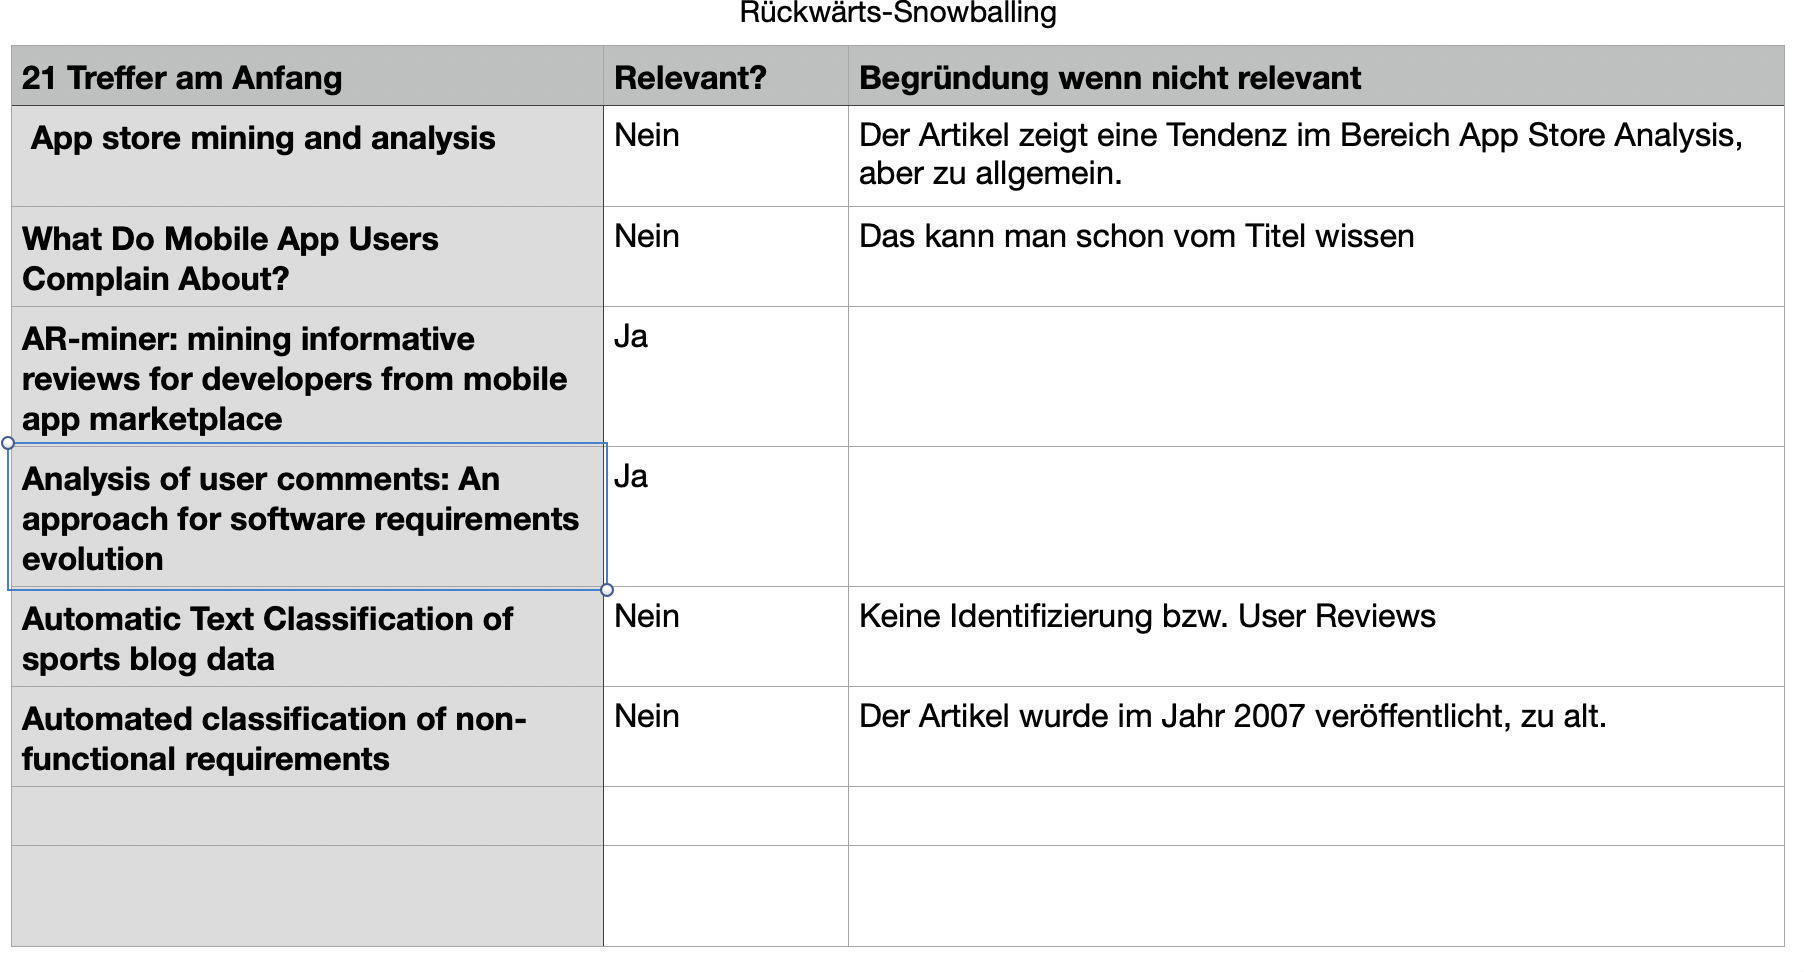
\includegraphics[scale=0.4]{../images/Thema1_BackwardSnowballing.png} 
\caption{Backward Snowballing Results}
\label{fig:model}
\end{figure}

In the IEEE platform there are 922366 results with the search term "Identification or Classification and Requirements and Review and “App Store”", and 4 from the first 50 results are relevant. And there are only 3 results with the search term "Classification and Requirements and Review and “App Store”" and 2 of them are relevant. In the ACM platform there are 88463 with the item "Identification and Classification and Requirements and Review" and 4 of them are relevant. 

\begin{figure}[H] 
\centering
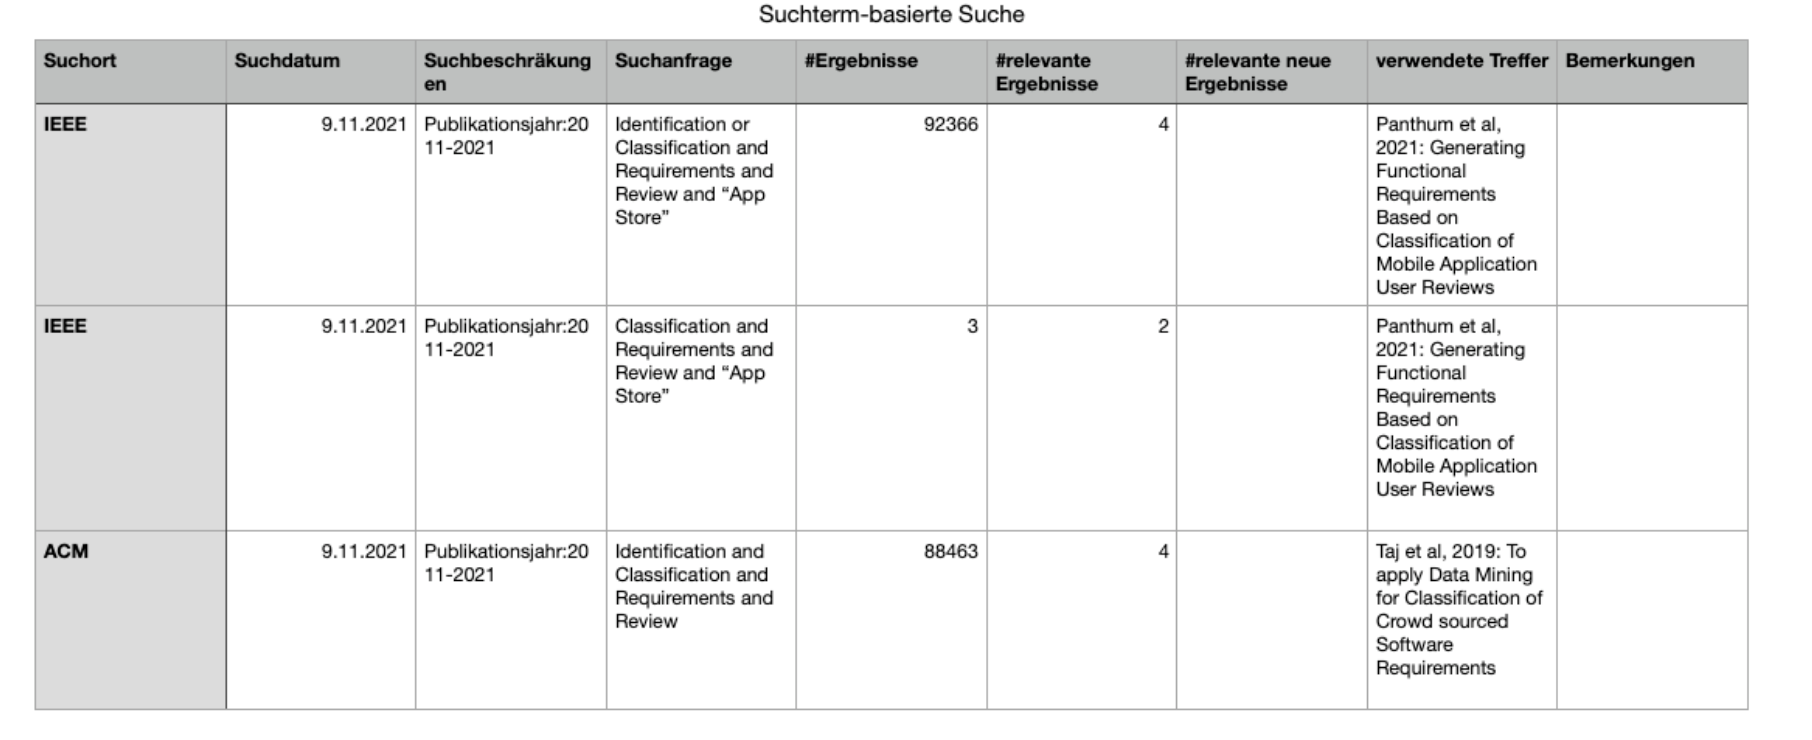
\includegraphics[scale=0.5]{../images/Thema1_TermBasedSearch.png}
\caption{Term-Based Search Results}
\label{fig:model}
\end{figure}

By reading and comparing the abstract some irrelevant papers can already be filtered out, but there are still 2 papers from the forward snowballing and two from the term based search. Then the second and third criteria has been applied to make the final decision which paper is more properly to be chosen. At the end, the found paper is ”Generating Functional Requirements Based on Classification of Mobile Application User Reviews.” Panthum et al.[2]. 


\chapter{Approach 1}

\section{Goal}
The aim of this approach is to automatically identify requirements from user reviews and to classify them into FRs and NFRs. FR stands for functional requirement and is what the system should do. NFR means non-functional requirement and describes how the system should work. A important part of NFR is quality requirement, which contains few parts on what people focus at most, e.g. usability, security or performance.

\section{Algorithm}
TF-IDF and NLP are used in this approach.\\
NLP: Natural Language Processing, which in this case is used to combine keywords to match user requirements from user reviews.

\subsection{TF-IDF}
TF-IDF: Term Frequency-Inverse Document Frequency, is statistically based in order to automatically extract key words of the requirements from the sample reviews. 

\begin{figure}[H] 
\centering
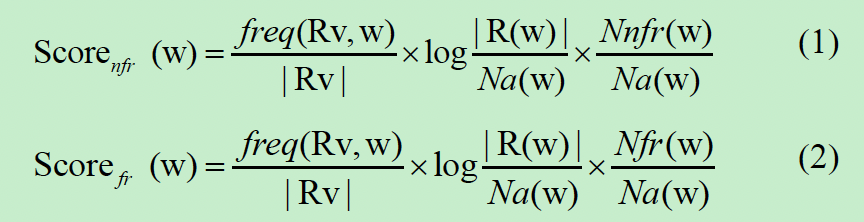
\includegraphics[scale=0.8]{../images/Thema1_TF_IDF.png}
\caption{TF-IDF}
\label{fig:model}
\end{figure}

\emph{Score(w)} represents the importance of the word \emph{w} in identifying and classifying user reviews.
TF-IDF has two sections: TF and IDF.
$$\frac{freq(Rv,w)}{|Rv|}$$ denotes the TF section. {|Rv|} refers to the quantity of all the words contained in the review \emph{Rv} and \emph{freq(Rv,w)} represents the frequency of word \emph{w} appearing in the sample review \emph{Rv}.
$$log\frac{|R(w)|}{Na(w)}$$ represents the IDF section, in which \emph{Na(w)} denotes the number of sample reviews that contain the word \emph{w} and |R(w)|denotes the number of reviews to be classified that contain the word \emph{w}. \emph{Nnfr(w)} or \emph{Nfr(w)} represents the number of NFR or FR sample reviews that contain the word \emph{w}.

\section{Evaluation}
The approach is evaluated through comparing automated classification results with manual classification results. \\
Recall is number of user reviews that are correctly classified as FRs divided by the number of user reviews containing FRs\\
Precision is number of user reviews that are correctly classified as FRs divided by the number of user reviews that are classified as FRs\\
F-measure could be calculated with Recall and Precision and will be used to measure the overall performance of the automated classification results. The results for the classification accuracy of NFRs and FRs are shown in figure 3.2. and figure 3.3. \\

\begin{figure}[H] 
\centering
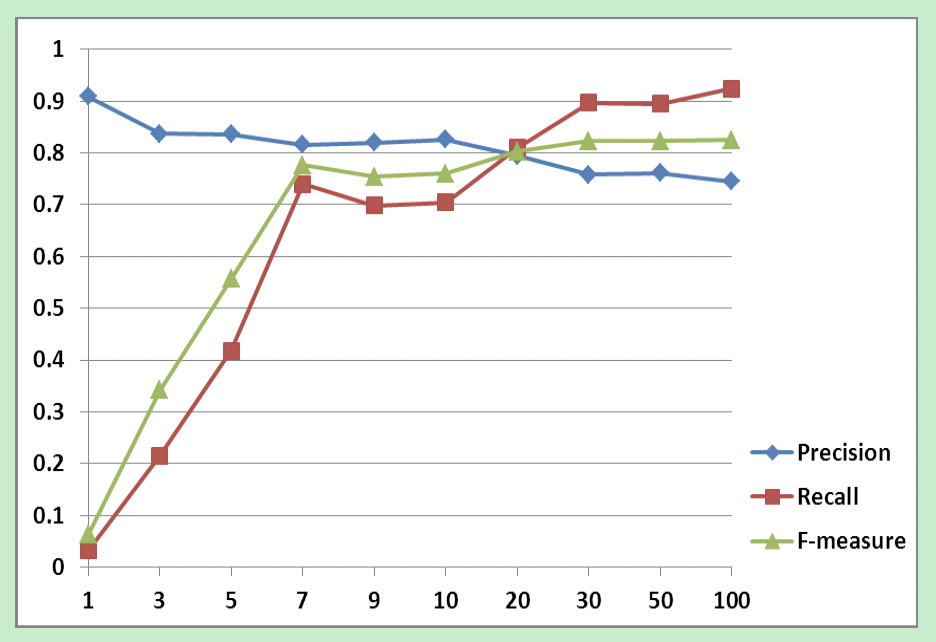
\includegraphics[scale=0.5]{../images/Thema1_NFR_Result.png}
\caption{NFR Result}
\label{fig:model}
\end{figure}
\begin{figure}[H] 
\centering
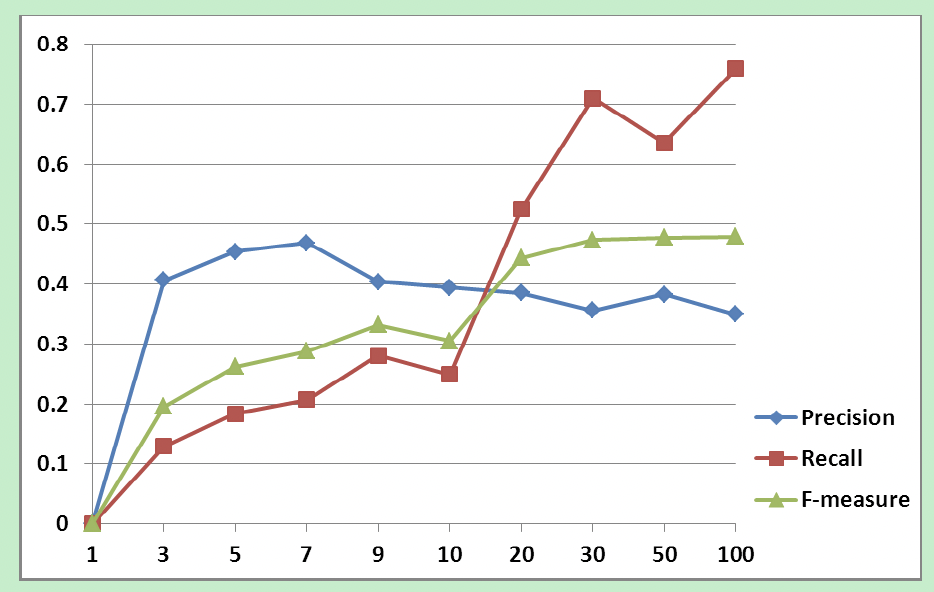
\includegraphics[scale=0.5]{../images/Thema1_FR_Result.png}
\caption{FR Result}
\label{fig:model}
\end{figure}
As one can see in figure 3.2 as well as in figure 3.3, the approach receives a relatively stable requirements classification with Precision, Recall and F-Measure with an appropriate size of sample reviews. 


\chapter{Approach 2}


\section{Goal}
The Goal of this approach is to generate functional requirements from the user reviews from app store and google play automatically.


\section{Algorithm}
Following some crucial parts of this approach are described with more detail. 

\subsection{Klassifikator Training}

\begin{itemize}
\item Stratified random sampling is used to split the dataset into a training set and a test set(in this paper 80:20).
\item SVMSMOTE is used to generate synthetic samples to handle imbalanced data.
\item Chi-Square is used for feature selection to reduce
the high dimension of textual feature.
\item MinMaxScaler is used for data normalization to adjust the
data to be in the same unit and comparable.
\item GridSearchCV is used for hyperparameter tuning to find optimal values for the hyperparameters of a model.
\end{itemize}

Naïve Bayes, Logistic Regression, Decision Trees, Random Forest algorithms are also used in the training applied.

\subsection{Clustering}
\begin{itemize}
\item Lemmatization and TF-IDF are used in the representation of the functional user reviews in the duplicate test set.
\item PCA is applied to reduce the dimensionality of the data.
\item Hopkins statistic is used to evaluate whether the data
contained meaningful clusters.
\end{itemize}
K-means, K-medoids, Hierarchical clustering, and DBSCAN algorithms are applied to the functional user reviews of each application. 

\subsection{Pairwise Text Similarity}
This method determines the similarity between each pair of functional user reviews. SBERT is used to generate sentence embeddings to represent functional user reviews. Sentence embeddings can capture textual content better than TF-IDF for semantic textual similarity. The similarity between each pair of functional user reviews was measured by Cosine distance. If the similarity between two functional user reviews is not less than the similarity threshold, then a duplicate is found.


\section{Evaluation}
The classifiers built in the experiment are evaluated in
terms of precision, recall, F1(F-Measure), and accuracy. The stratified 10-fold cross validation is applied to train classifier with others together, then test set are used to evaluate the classifiers.

\begin{figure}[H] 
\centering
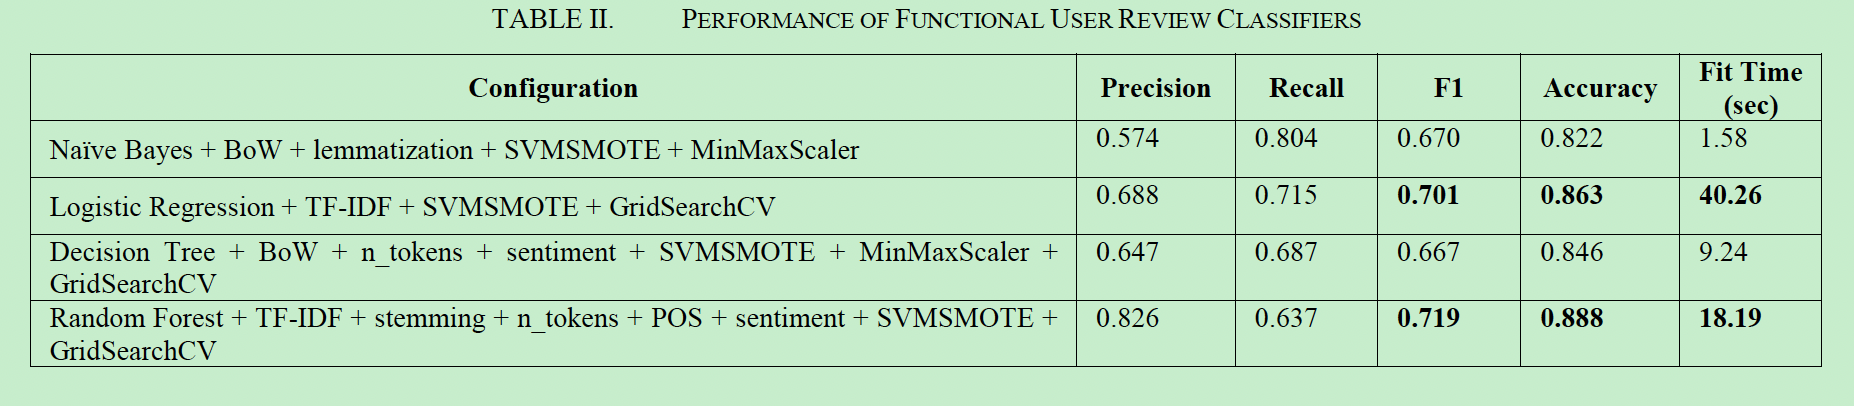
\includegraphics[scale=0.5]{../images/Thema1_ClassifierPerformance.png}
\caption{Classifier Performance}
\label{fig:model}
\end{figure}
As can be seen from the table, among the classifiers,
the last combination has the best performance at 71.9 \% F1 and 88.8\% accuracy.

To evaluate the quality of the functional requirements, functional requirements are generated from 1808 sets of functional user reviews. Five requirement boiler plates and 13 review templates are involved. And at last 48 functional requirements are generated.

\chapter{Comparision}
\section{Summary}

The first article is "Identification and Classification of Requirements from App User Reviews." Yang et al.\cite{YangLiang2015}.
The second article is "Generating Functional Requirements Based on Classification of Mobile Application User Reviews." Panthum et al.\cite{PanthumSenivongse2021}.

User reviews are important resources for developers to get feedback for making improvements. So it makes sense to analyse and identify the critical user needs. But with the huge amount of user reviews, how to do it more effectively becomes a challenge. In the first paper, an approach is presented to automatically identify requirements and classify them into two categories using TF-IDF and NLP techniques with human intervention in keywords selection for requirements identification and classification. The results show that the approach receives a relatively stable requirements classification containing precision, recall, and F-measure with an appropriate size of sample reviews, which is meaningful and practical for APP developers to elicit requirements from user reviews.

User reviews are also important resources for developers for maintaining and evolving applications. Since there are lots of user reviews, it is cumbersome to go through all user reviews to identify useful information for further maintenance and evolution. The second paper proposes an initial attempt for automating the generation of
functional requirements from user reviews on the App Store and Play Store using machine learning and NLP techniques. The results shows that the generated functional requirements obtained moderate to high scores in terms of readability, unambiguity, completeness, and validity. The proposed approach can help the development team identify functional requirements from direct feedback of the users.

\section{Synthesis}

\subsubsection{Name of the approach}

The name is not specially mentioned, so "The approach by Yang et al." will be used.

\subsubsection{Description of the approach}

This approach can automatically identify requirements and classify them into FRs and NFRs using TF-IDF and NLP technique with human intervention in keywords selection for requirements identification and classification.
TF-IDF is used to automatically extract requirement keywords from the sample reviews.
NLP(regular expression) is used to match user requirements from user reviews in Phase: Identify and Classify Reviews.
Human interventions exist in manual requirements classification by experts for sample reviews and keywords selection.

\subsubsection{Benefits  of the approach}
The step for app developers to elicit requirements from user reviews is supported by the approach.

\subsubsection{Tool support for the approach}
There are two components of a tool: User Reviews Extractor and Requirements Identifier and Classifier. User Reviews Extractor is used to extract and collect user review information from APP platforms as raw data to be further processed, and Requirements Identifier and Classifier is used to identify and classify requirements from user reviews into FRs and NFRs, which has 5 phases: 1.Input user reviews 2.Pre-process User Reviews 3.Extract Keywords 4.Combine Keywords 5.Identify and Classify Reviews
In Phase 3 experts do a manual requirements classification first.

\subsubsection{Evaluation of the approach}
The approach is evaluated through comparing automated
classification results with manual classification results and F-measure is used to measure the overall performance of the automated classification results. And the results show that the approach receives a relatively stable requirements classification containing precision, recall, and F-measure with an appropriate size of sample reviews.

\subsubsection{Name of the approach}
The name is not specially mentioned, so "The approach by Panthum et al." will be used.

\subsubsection{Description of the approach}
This approach can automatically generate functional requirements from user reviews on the App Store and Play Store using machine learning and NLP technique. 
Stratified random sampling is used to split the dataset into
a training set and a test set.
SVMSMOTE is used to generate synthetic samples to handle
imbalanced data.
Chi-Square is used for feature selection to
reduce the high dimension of textual feature.
MinMaxScaler is used for data normalization to adjust the data to be in the same unit and comparable.
GridSearchCV is used for hyperparameter tuning to find optimal values for the hyperparameters of a model.
Naïve Bayes, Logistic Regression, Decision Trees, Random Forest algorithms are also used in the training applied.
Clustering is a technique to segregate data into different
groups.
Lemmatization and TF-IDF are used in the representation of the functional user reviews in the duplicate test set.
PCA is applied to reduce the dimensionality of the data.
Hopkins statistic is used to evaluate whether the data contained meaningful clusters.
K-means, K-medoids, Hierarchical clustering, and DBSCAN algorithms are applied to the functional user reviews of each application.
SBERT is used to generate sentence embeddings to represent functional user reviews.



\subsubsection{Benefits  of the approach}
Maintenance and evolution process of a mobile development team can be supported by the approach.

\subsubsection{Tool support for the approach}
App-store-scraper and google-play-scraper are used to screen-scrape user reviews of the applications in the similar categories to the ones selected by other researches. Requirement boilerplates are used to generate functional requirements.

\subsubsection{Evaluation of the approach}
Functional user reviews are generated from functional requirements to evaluate the functional requirements quality.
The result shows that the generated functional requirements obtained moderate to high scores in terms of readability, unambiguity, completeness, and validity.

\section{Synthesis Matrix}
\begin{table} [H] 
\centering
\begin{small}
\caption{Synthesis matrix }
\label{tab:table}
\setlength{\tabcolsep}{1em}
\begin{tabular}{ p{2cm}| p{3cm} | p{3cm} | p{3cm} }
\hline
 \textbf{Nr.synthesis question}&\textbf{ Name}&\textbf{Hui Yang, Peng Liang}&\textbf{Tanutcha Panthum, Twittie Senivongse}\\
\hline
 \hline	
  3a) & Used Methods & TF-IDF and NLP & SVMSMOTE, Chi-Square, MinMaxScaler, GridSearchCV, Naïve Bayes, Logistic Regression, Decision Trees, Random Forest, Lemmatization and TF-IDF, PCA, Hopkins statistic, K-means, K-medoids, Hierarchical clustering, DBSCAN, SBERT \\
 \hline
  3b)& Classification Goal & FRs and NFRs & Generation of FRs  \\
 \hline
  3c) & Data requirements and limitations & human intervention & / \\
  \hline	
  4a) & Supported Development Processes & Requirements Elicitation & Requirements Elicitation\\
 \hline
  4b) & Supported Stakeholders & Developers & Developers  \\
 \hline
  5a) & Tool support / Prototype & User Reviews Extractor and Requirements Identifier and Classifier & App-store-scraper, google-play-scraper, requirement boilerplates\\
  \hline	
  5b) & Degree of Automation & medium, human interventions exist in sample reviews and keywords selection & high\\
 \hline
  6a) & Evaluation & Comparing automated/manual classification in F-measure & Readability of generated functional user requirements  \\
 \hline
  6b) & Evaluation results & F-Measure 0.825 for NFR and 0.479 for FR sample reviews 100 & Readability 3.99 Unambiguity 3.15 Completeness 3.20 Validity 3.11 \\
  \hline
\end{tabular}
\end{small}
\end{table}


\section{Differences and Similarities}
Both articles focus on identification and classification requirements from the user reviews from app store. However the article by Yang et al. uses the TF-IDF and NLP as main methods to identify user reviews and classify them into NFRs and FRs, while the article by Panthum et al. uses machine learning methods and NLP to finally generate FRs. The data processing in the article by Panthum et al. is more in detail comparing to the article by Yang et al.. Requirements identification and classification in the given article is performed in one step based on requirement keywords set using TF-IDF. Nevertheless, classifier is trained first using different configurations in the article by Yang et al.. There is also a part for duplicate requirements detection in the article by Panthum et al. using clustering and text similarity. Finally the functional requirements are generated using sentence pattern matching and requirements boilerplates. 'User reviews' are done at a sentence level, that means each user review was split into sentences.

\chapter{Conclusion} 
Both articles focus on identification and classification requirements from the user reviews from app store. However the article by Yang et al. uses the TF-IDF and NLP as main methods to identify user reviews and classify them into NFRs and FRs, while the article by Panthum et al. uses machine learning methods and NLP to finally generate FRs. The data processing in the article by Panthum et al. is more in detail comparing to the article by Yang et al.. Requirements identification and classification in the given article is performed in one step based on requirement keywords set using TF-IDF. Nevertheless, classifier is trained first using different configurations in the article by Yang et al.. There is also a part for duplicate requirements detection in the article by Panthum et al. using clustering and text similarity. Finally the functional requirements are generated using sentence pattern matching and requirements boilerplates. "User reviews' are done at a sentence level, that means each user review was split into sentences.




